\chapter{Component Framework}
\label{chapter:osgi}

To address the requirements described in Chapter \ref{chapter:requirements}, the ``Component
Framework'' has been developed as part of this master thesis. As the underlying technical basis the
OSGi Framework is used.

Section \ref{sec:osgi} therefore introduces the ``OSGi Service Platform'', which forms the basis for
the Component Framework and is specified by the ``OSGi Alliance'' \cite{osgi-alliance}. The OSGi
Alliance is a worldwide consortium of technology innovators, which assures interoperability of
applications and services based on the OSGi Service Platform.

% Implementations of the OSGi Service Platform therefore provide means to install bundles, services and
% additional functionality respectively at runtime. That means that a running application, which is
% based on this platform, can be extended with further functionality, without restarting it.

Having the necessary background information, Section \ref{sec:component_framework} finally describes
the developed ``Component Framework'' in detail. It explains the functionality that was obtained by
the OSGi Service Platform as well as the extensions or adaptations that were implemented to realize the
requirements introduced in Section \ref{chapter:requirements}, like extensibility, running multiple
instances of a block, grouping of blocks, reusability of groups, event management and logging.

\section{OSGi Service Platform}
\label{sec:osgi}

This section introduces the OSGi Service Platform which has been used as underlying technical basis
for the development of the Component Framework.

The ``OSGi Service Platform'' is a dynamic module system for Java that allows the dynamic integration
and remote management of bundles (i.e., a cohesive unit of classes and resources) and services.
Furthermore, the service platform offers means to install, start, stop and uninstall bundles and
services at runtime without stopping and restarting the platform as a whole.\newline The
specification of the OSGi Service Platform is publicly available and can be accessed via the website
of the OSGi Alliance \cite{osgi-alliance}. The current version of the specification is 4.1 and
consists of three major parts, namely the ``Core Specification'', the ``Service Compendium and the
``Mobile Specification''.

\noindent\textbf{\textit{Core Specification:}}\newline The Core Specification
defines the OSGi Framework and Framework Services which are based on it. The OSGi
Framework is the base component of the Service Platform and provides the
infrastructure for installing, starting, stopping and uninstalling bundles and
services.

\noindent\textbf{\textit{Service Compendium:}}\newline The Service Compendium
includes a series of standard services, which are built on top of the OSGi
Framework and provide special functionality for various use cases. Examples of
standard services are a logging or configuration service as well as an event
service, which provides an interface for handling events throughout the
framework.

These services can be loaded at system startup or installed at runtime and are
registered at the service registry, where they can be accessed by every bundle
and service throughout the whole framework.

\noindent\textbf{\textit{Mobile Specification:}}\newline The Mobile Specification
includes a subset of the services, which are specified by the Service Compendium,
and adds some special services for mobile devices, which are also built on top of
the core specification.

\subsection{OSGi Framework}
\label{label_osgi_framework}
The cornerstone of the OSGi service platform is the ``OSGi Framework'' which
constitutes a container for bundles and services.

A \textbf{bundle} is a cohesive unit of classes and resources which can be
installed and uninstalled in the framework. These classes and resources are not
visible to other bundles initially. In order to make them visible and therefore
usable for other bundles, the packages containing the classes and resources, have
to be exported explicitly. Similarly, bundles which want to use the exported
packages have to import these. This mechanism enables a loose coupling between
the various bundles.\newline As soon as a bundle is installed in the OSGi
Framework, it tries to resolve the dependencies and to allocate the needed
packages respectively. If the required packages are not available in the system,
the bundle can not be started.

Another means of decoupling and service orientation is the ability of bundles to
use \textbf{services}. These services are Java-objects which are registered with
their interface-names at the so-called ``Service Registry''. This service
registry is available throughout the whole framework. Therefore, other bundles
can query the registry and obtain a service for further usage. No information
about the implementation or about the bundle that exposes the service is needed.

Finally, the \textbf{Management Agent}, which is part of the OSGi Framework,
enables the administration of bundles. In a very basic form this management agent
provides a text-based console which offers possibilities to install, uninstall,
start and stop bundles at runtime.

\subsection{OSGi Framework Specification}
The specification of the OSGi Framework is subdivided into multiple logic layers
(see Figure \ref{fig:osgi_framework_logic_layers}):

\begin{figure}
	\centering
		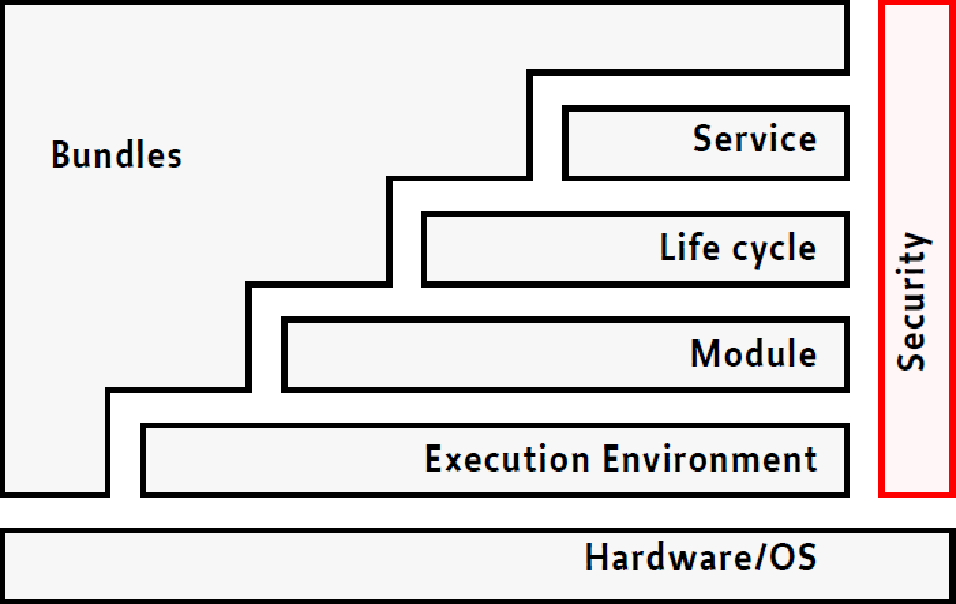
\includegraphics[width=0.8\textwidth]{Bilder/osgi-framework.pdf}
	\caption{OSGi Framework - Logic Layers}
	\label{fig:osgi_framework_logic_layers}
\end{figure}

\subsubsection{Execution Environment}
The OSGi Framework is specified in a way that enables the execution on various
Java-platforms. Therefore so-called ``Execution Environments'' are defined. These
execution environments are representations of concrete Java-runtimes, which
constitute the needed classes, interfaces and methods.

Two execution environments are specified in the Service Compendium:
\begin{itemize}
  \item The \textbf{OSGi/Minimum-1.1} defines the minimal environment that is needed for the
  execution of the OSGi Framework and the general services.
  \item A superset of the OSGi/Minimum-1.1 execution environment is the
  \textbf{CDC-1.0/Foundation-1.0}, which is a derivation of the JME Foundation Profile
  \cite{jme_foundation_profile}.
\end{itemize}

Based on the given premises concerning hardware, processing power and memory
resources the adequate execution environment has to be chosen.

But not only the OSGi Framework itself specifies the execution environment it
needs, also single bundles can specify a special execution environment. If such
a bundle is to be installed in the OSGi Framework it is checked if the given
execution environment satisfies the bundle's specification. If this is the case
the bundle is installed.

\subsubsection{Module-Layer:} \label{paragraph_module_layer} The module-layer
defines the bundle as the basic modularization-unit within the OSGi Service Platform. Technically, a bundle is
nothing else than a Java-archive, which contains the classes and resources for
the implementation of the functionality that should be provided by this
bundle.\newline Additionally, a bundle includes a ``Manifest''-file (see Figure
\ref{fig:manifest}), which contains various information about the bundle,
described in a declarative way. This information is needed by the framework to
run the bundle correctly.\newline The symbolic name and the version information,
for example, are needed to explicitly identify a bundle within the OSGi Service
Platform.\newline Also the dependencies between bundles, described in Section
\ref{label_osgi_framework}, are defined in the Manifest-file.

\begin{figure}
	\centering
		\fbox{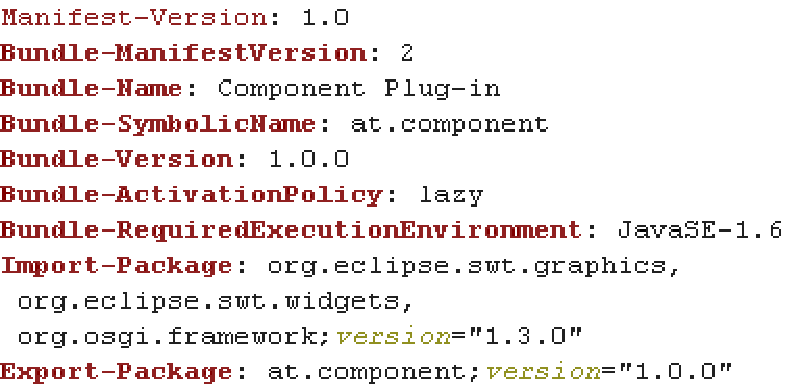
\includegraphics[width=0.8\textwidth]{Bilder/manifest.pdf}}
	\caption{MANIFEST.MF example}
	\label{fig:manifest}
\end{figure}

\subsubsection{Life-Cycle-Layer:}
\label{label_life_cycle_layer}
While the module layer describes the static aspects of bundles, the
life-cycle-layer specifies the dynamic ones.\newline
It defines the various states (see Figure \ref{fig:life_cycle_states}) a bundle
can have and the conditions and actions, which can lead to a state-change. In order to manipulate
the states of a bundle a so-called ``Management Agent'' implements an interface to the OSGi
Framework, which allows to control the framework from the outside.
Therefore, a Management Agent can provide a simple console for firing commands or a more
complex user interface, which provides various administrator tools.\newline
The installation of a bundle is one of the four basic operations a
management agent supports. If a bundle is installed successfully in the framework it is in the
``INSTALLED'' state. As soon as the framework has resolved all
package-dependencies it moves to the ``RESOLVED'' state.\newline
As a second operation the management agent implements the functionality to
start a bundle, which leads to the ``ACTIVE'' state on success or to the
``RESOLVED'' state otherwise. The stop-operation leads to the ``STOPPING''
state and to the ``RESOLVED'' state as soon as the stopping-operation is
finished.\newline
Finally the fourth operation enables the uninstalling of the bundle, which
requires a ``INSTALLED'' or ``RESOLVED'' state. If the bundle is in ``ACTIVE''
state the stop-operation has to be called at first.\newline
In addition to the four basic operations the framework provides the
possibility to update or refresh a bundle, which provides the opportunity to
exchange a bundle with a different version of the same bundle.


\begin{figure}
	\centering
		\fbox{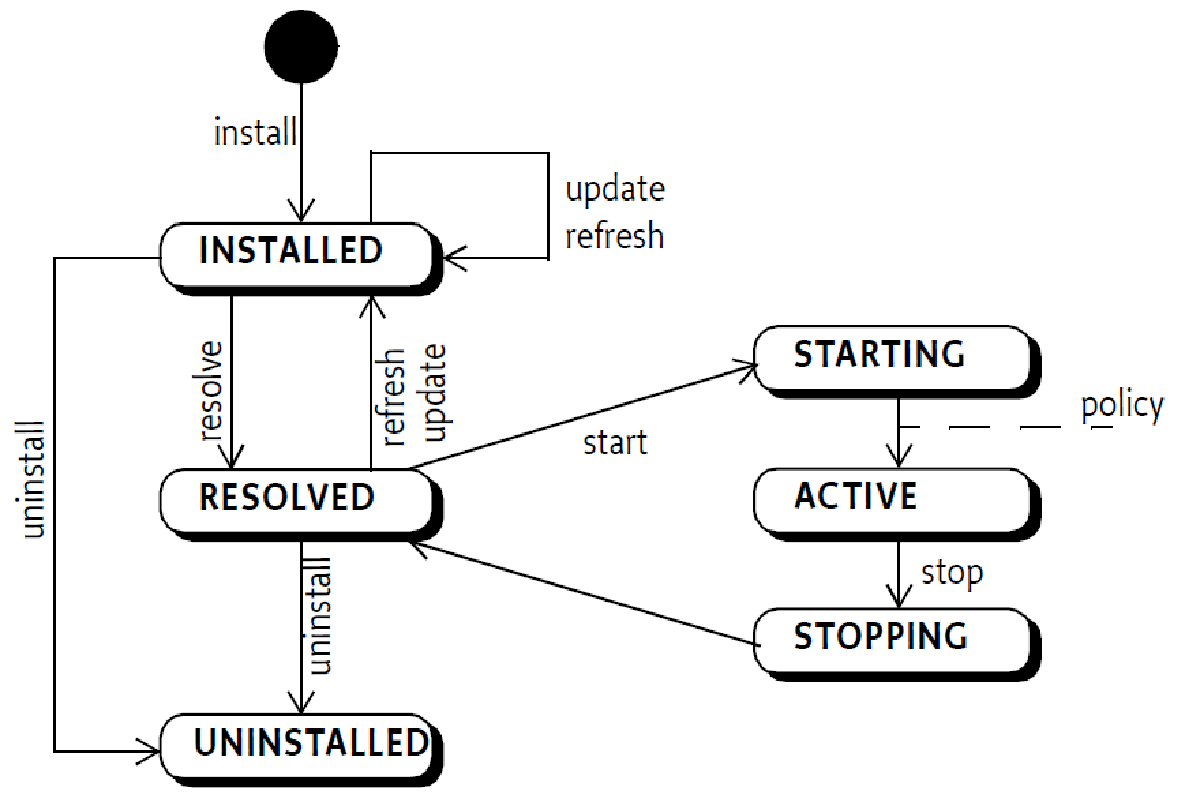
\includegraphics[width=0.8\textwidth]{Bilder/bundle-states.pdf}}
	\caption{Life-Cycle-States}
	\label{fig:life_cycle_states}
\end{figure}

\subsubsection{Service-Layer:}
\label{sec:service_layer}
The Service-Layer specifies a general Service-Model which makes services
available throughout the OSGi Framework. This model is implemented via a ``service
registry'', which constitutes the central point for registering, querying and
unregistering services.

As described in Section \ref{label_osgi_framework}, a ``Service'' is a simple
Java-object, which is registered at the service registry via it's interface-name.
Bundles that want to use this service can query the registration via the
interface-name and use the service. These bundles are called ``service consumers''
and do not know anything about the implementation details of a service. A
further detail that should be mentioned here is the possibility of having
multiple services implementing the same interface. Hence, the service consumer faces the
choice of using either one of the multiple services or all of them in parallel.

As services within the OSGi Framework can be registered and unregistered at any
time, a service consumer also has to anticipate the absence of a service and
provide sufficient error handling functionality. In order to alleviate the
handling of the described situations, the OSGi specification describes
possibilities like the``Service Tracker'', which provides means for detecting,
accessing and finally using registered services for a given service interface
name and wraps the complexity of directly using the service registry. 

The standard way of providing services is to set up one bundle that includes the
interface for a service and a second bundle that provides the implementation of
the interface and the service respectively. This scheme reduces dependencies and
allows the exchange of the service implementation at runtime.

A bundle that implements a new service and registers it at the service registry
is therefore called ``service producer''.

\subsubsection{Security Layer:}
The security layer is based on the Java 2 security architecture and provides
means for constraining execution rights for every single bundle. The support
for this security concept within an OSGi implementation is optional.

\subsection{OSGi Standard Services}
\label{sec:standard_services}
Based on the OSGi Framework Specification the OSGi Service Platform Service
Compendium and the OSGi Service Platform Mobile Specification define a series
of Standard Services, which provide solutions for various problems.\newline
The following service descriptions are only an excerpt of the full
specification and include only the services which can be associated with the
implemented application (see Section \ref{sec:component_framework}).

\noindent\textbf{\textit{Event Admin Service:}} The Event Admin Service
provides a mechanism for propagating events between bundles throughout the whole
framework. As an event can be identified by it's unique ``Topic'' every bundle
can specify an ``Event Handler'' for each of these topics.

\noindent\textbf{\textit{Wire Admin Service:}} In order to connect two services
at runtime the Wire Admin Service is needed. Each service can take the role of
an information consumer and/or producer and can exchange data via the
established connection.

\noindent\textbf{\textit{Application Admin Service:}} The Application Admin
Service empowers the OSGi Framework to manage external applications. Via the so
called Application Admin these applications can be for example started and
stopped.

\noindent\textbf{\textit{Log Service:}} The Log-Service specification implements
services for writing log-information like warnings, errors or debug-information.

\noindent\textbf{\textit{Configuration Admin Service:}} If services have to be
configured at runtime, the Configuration Admin Service is considered the best.

\noindent\textbf{\textit{Metatype Service:}} This service provides means for
adding meta-information to services, which can be queried and interpreted at
runtime. In connection with the Configuration Admin Service a ``Management Agent''
can use this information to provide a user interface for the configuration of a
service.

\noindent\textbf{\textit{Preference Service:}} The Preference Service implements the access to a
simple, hierarchic database, where bundles can store and read system- and user information.

\noindent\textbf{\textit{User Admin Service:}} This service specifies the
authorization and authentication of users, based on user- and group information.
Therefore, bundles can check if a specific user can access a certain
functionality.

\noindent\textbf{\textit{Declarative Service:}} With the help of this service a
bundle can declaratively define components with it's service-dependencies. The
so-called ``Service Component Runtime'' manages these components and dependencies
at runtime. Therefore a bundle does not have to manage the required services
anymore.

\subsection{OSGi Implementations}
\label{sec:osgi_implementations}

Several OSGi implementations are available and are therefore introduced in the following sections.

\subsubsection{Open Source Implementations}

\begin{itemize}
	\item\textbf{Eclipse Equinox}\newline Eclipse Equinox founds the basis for all Eclipse-applications
	and the Eclipse-IDE itself. Therefore Equinox is the commonly used OSGi Platform on the desktop.
	\item\textbf{Prosyst mBedded Server Equinox Edition}\newline This implementation of the OSGi
	Platform is available since March 2007, is based on Eclipse Equinox and provides, among others,
	additional standard services. Meanwhile Prosyst joined the Eclipse Foundation and is actively
	involved in the development of Equinox.
	\item\textbf{Knopflerfish}\newline Knopflerfish is developed by ``Makewave'' and provides an
	implementation of the OSGi-R4-specification.
	\item\textbf{Apache Felix}\newline Since 2007 Felix is one of the top-level-projects of Apache.
	Felix is based on the older OSGi implementation, called ``Oscar'' and is licensed under the
	``Apache License 2.0''.
\end{itemize}

\subsubsection{Commercial Implementations}

\begin{itemize}
	\item\textbf{Knopflerfish Pro}\newline Knopflerfish Pro is the commercial variant of Knopflerfish
	and extends the open source implementation with various drivers for GPS-devices and the serial
	COM-interface.
	\item\textbf{Prosyst mBedded Server Professional Edition}\newline Besides the open-source version
	Prosyst also provides the commercial mBedded Server Professional Edition. It is especially
	optimized toward performance and memory requirements. Therefore, it is qualified for platforms with
	very limited resources.
\end{itemize}


\section{Component Framework}
\label{sec:component_framework}

This section describes the ``Component Framework'', which has been implemented as part of this
master thesis and constitutes a proof-of-concept implementation. The framework is based on Java and
the described OSGi Service Platform and realizes the requirements introduced in Section
\ref{chapter:requirements}. Therefore, it provides an infrastructure or framework for developing,
managing, displaying and connecting so-called components. A component is the basic building block of
the Component Framework and is introduced in the next section.

\subsection{Components - The major Building Blocks of the Component Framework}
\label{sec:component}

A component within the Component Framework can be compared to blocks within the mashup composer
tools.

In more technical words a component is nothing else than a service which is implemented and
registered by an OSGi bundle (see Section \ref{label_osgi_framework}). In order to make the
component service seamlessly integrable into and manageable by the Component Framework it has to
implement a predefined service interface.

As soon as the service is registered at the service registry it is accessible throughout the entire
framework and the necessary methods to display the component user interface within an application
can be invoked. Moreover, the Component Framework enables the distinction between ``normal''
components and more complex components, which can have ``child-components'' allowing the grouping
of components (see Section \ref{sec:project}).

Summing up, a component is an application with a user interface, which is managed and displayed by
the Component Framework.

\subsection{Grouping of Components (Requirements 5 and 6)}

As one of the major requirements for the Component Framework was Requirement 5 ``Grouping of
Blocks'' (see Section \ref{chapter:requirements}), this section introduces the various grouping
methods which are included in the Component Framework.

The grouping of blocks requirement describes two different methods. The concept of ``projects''
realizes the first method which is responsible for displaying multiple user interfaces, which are
easily switchable and the concept of ``complex components'' realizes the second method and hence
provides means to display multiple groups of components on a single user interface.

\subsubsection{Projects - Containers for Components}
\label{sec:project}
To realize the requirement of multiple user interfaces, which are easily switchable, the concept of
``projects'' was introduced. For this purpose, a hierarchical structure was implemented, which means
that each component has a parent component and possibly one or multiple child components. The only
component that has no parent is the so-called project-component, which is the top-level component of
a project. As the Component Framework's intention is to enable the simple composition of
applications, the definition of projects and the introduction of a component hierarchy extend the
framework with the functionality of editing multiple projects or applications respectively in
parallel and grouping components on multiple sites according to their logical connection.

Furthermore, the Component Framework enables the saving and deploying of projects, which fulfills
Requirement 6 ``Reusability of Groups''.

\subsubsection{Complex Components}
\label{sec:complex_components}
The requirement of displaying multiple groups of components on a single user interface was realized
by introducing so-called ``complex components''. As described previously the Component Framework
introduces a parent child relationship between components. A complex component therefore is a
component which can have multiple child components and can be used as a top-level component for the
project (see Section \ref{sec:project}). The ``Group'' and ``Tabfolder'' components which were
implemented for the prototype application are examples for such components.

Figure \ref{fig:project_structure} finally depicts the overall structure of a project, which can be
compared to the well-known ``composite pattern'' \cite{GammaHelmEtAl95}.

\begin{figure}
	\centering
		\fbox{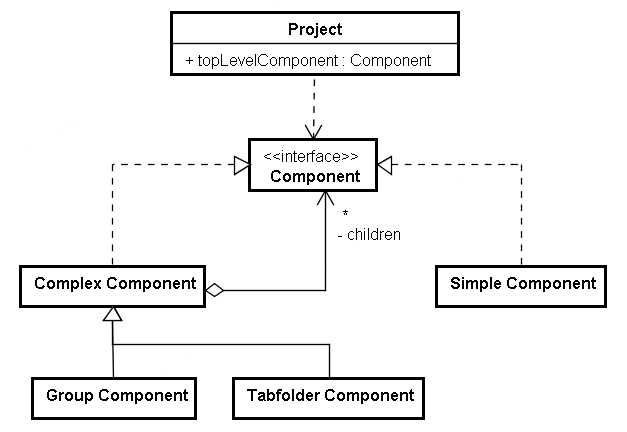
\includegraphics[width=0.98\textwidth]{Bilder/project-diagram.png}}
	\caption{Component Framework - Structure of a Project}
	\label{fig:project_structure}
\end{figure}

Figure \ref{fig:framework_ui} shows the realization of the project within the prototype
application. The red rectangle shows the project-component, the blue rectangle enframes the
so-called ``Group'' component (see Section \ref{sec:complex_components}), which can have multiple
child components and every green rectangle constitutes a simple component.

\begin{figure}
	\centering
		\fbox{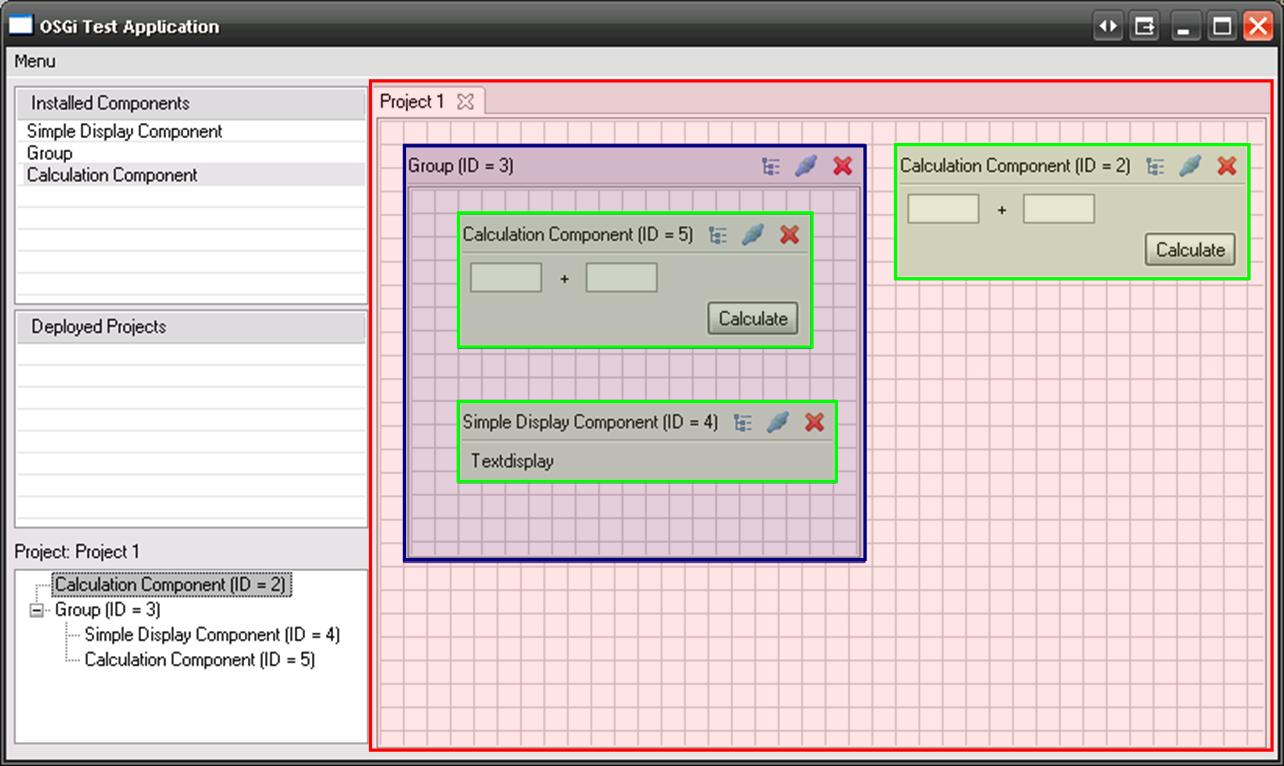
\includegraphics[width=1.2\textwidth,
		angle=90]{Bilder/framework_ui.jpg}}
	\caption{Component Framework - User Interface}
	\label{fig:framework_ui}
\end{figure}

\paragraph{Group Component}
The group component provides a working area where child components can be dropped and arranged
within a grid. Furthermore, it attaches a menu bar to each child component and provides
possibilities to drag and drop child components to other group components and to resize and rename every child component. The
items within the menu bar furthermore enable the configuration of connections to other components
(see Section \ref{sec:wire_admin}), the display of information about events which are
published by the child component (see Section \ref{sec:event_admin}) and the stopping
of the component.\newline
The goal of implementing such a component was to provide a work-area similar to those of the
inspected mashup tools (cf. Requirement 1 ``Simple User Interface'').

Figure \ref{fig:group_component} depicts a group component with a single child component, which
again is a group component.

\begin{figure}
	\centering
		\fbox{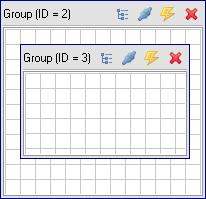
\includegraphics{Bilder/group_component.jpg}}
	\caption{The Group Component}
	\label{fig:group_component}
\end{figure}

\paragraph{Tabfolder Component}
The tabfolder component provides, as the name implies, a tabfolder which can hold multiple child
components as tabitems. Again, the child components can be added by simply dropping them from the
catalog into the tabfolder. The component also provides a menu bar which provides methods for
renaming the currently selected child component as well as connecting it to other components (see
Section \ref{sec:wire_admin}).

Figure \ref{fig:tabfolder_component} depicts a tabfolder component with two child components,
namely a group and a tabfolder component.

\begin{figure}
	\centering
		\fbox{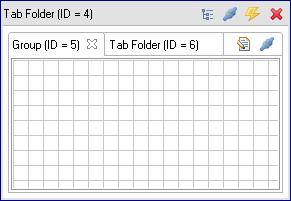
\includegraphics{Bilder/tabfolder_component.jpg}}
	\caption{The Tabfolder Component}
	\label{fig:tabfolder_component}
\end{figure}

As the working area and the tabfolder container are provided by single components and the Component
Framework is extensible (see Section \ref{sec:extensibility}) it is quite easy to either customize
the existing complex components and therewith create an individual working area or to extend the
framework with new components, which, for example, provide a user interface for dropping components
into a table or menu bar (cf. Requirement 3 ``Extensibility'').

\subsection{Services of the Component Framework}

This section describes the services which were implemented for the Component Framework to realize
Requirement 2 ``Data Access and Processing'', Requirement 4 ``Running multiple Instances of a
Block'', Requirement 7 ``Hot Deployment and Life-cycle Management'', Requirement 8 ``Event
Management'' and Requirement 9 ``Logging''.

The services of the Component Framework include the Component Starter Service, which is responsible
for starting multiple instances of a component, a simple ID service, which provides a unique ID
within a project of the Component Framework, extensions for the Wire Admin and Event Admin services
which enable data exchange and communication between components, and the powerful Component Service
which is responsible for managing the life-cycle of simple and complex components as well as
projects.

\subsubsection{Introduction: The OSGi Framework as Basis for the Component Framework}
The basis of the Component Framework is formed by the implementation of the OSGi Framework provided
by Eclipse, called ``Equinox''. This framework integrates the functionality to install, start, stop
and uninstall bundles that implement a component at runtime as well as to register services at the
service registry. Thereby, the OSGi Framework provides a good basis to fulfill Requirement 4
``Running multiple Instances of a Block'' and Requirement 7 ``Hot Deployment and Life-cycle
Management''.

Furthermore, Eclipse Equinox integrates multiple services which are contained in the OSGi Standard
Services specification (see Section \ref{sec:standard_services}) and provide the functionality to
communicate and exchange data between services and components respectively and are hence adapted for
the usage with components within the Component Framework.

\subsubsection{Component Starter and ID Service (Requirement 4)}
\label{sec:component_starter_service}
One of the major requirements for mashup composers and for the Component Framework is the possibility
to launch multiple instances of a component (cf. Requirement 4 ``Running multiple Instances of a
Block''). To realize this requirement the Component Framework integrates the Component Starter and
the ID Service.

\paragraph{The Component Starter Service}
As mentioned before components are implemented and registered by OSGi bundles which are installed
and started within the OSGi Framework. During the starting process of such a ``component bundle''
the Component Starter Service is registered at the service registry. As soon as the framework is up
and running and the first component is added to the working area, this service is requested in
order to instantiate and register a new instance of the component (see Figure
\ref{fig:registering_component_instances}).

\begin{figure}
	\centering
		\fbox{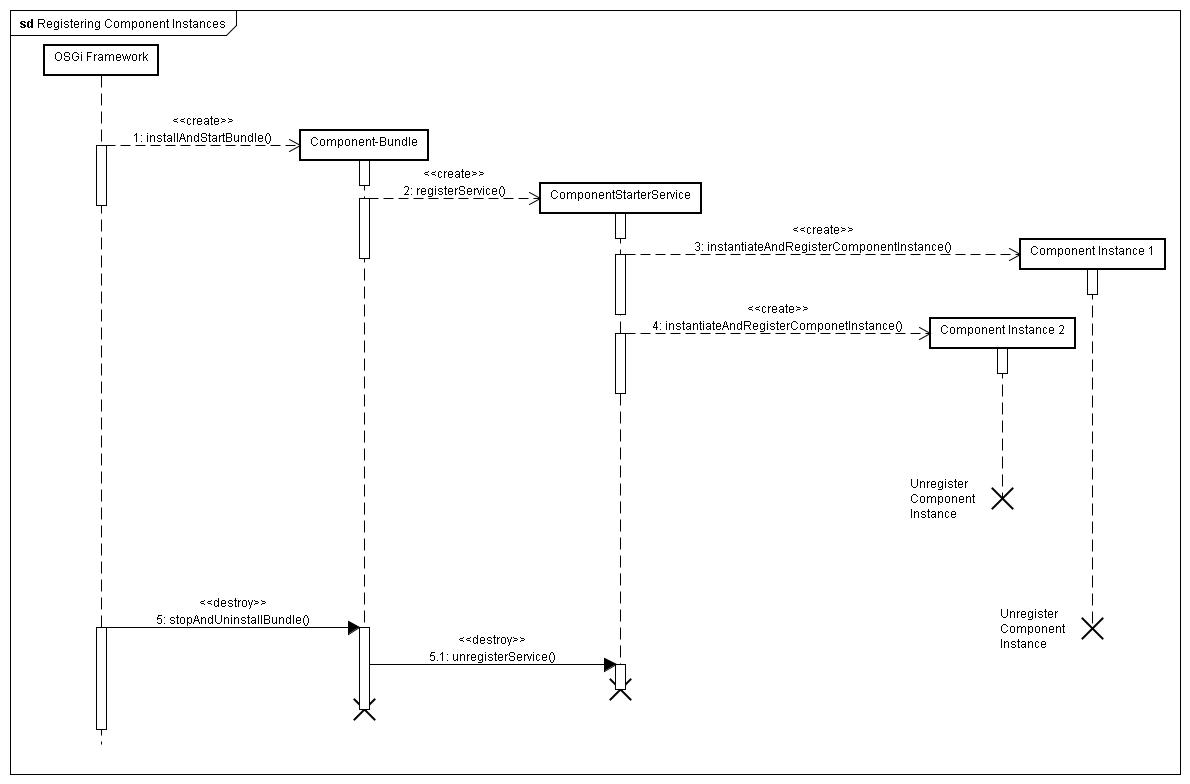
\includegraphics[width=1.2\textwidth,
		angle=90]{Bilder/sd_registering_component_instances.jpg}}
	\caption{Registering Component Instances}
	\label{fig:registering_component_instances}
\end{figure}

\paragraph{The ID Service}
\label{sec:id_service}
This service enables the unique identification of every instantiated and registered component
within the Component Framework, which is not provided by the OSGi Framework, but needed to realize
the ``Running multiple Instances of a Block'' requirement.

Within the OSGi Framework each bundle is identified by its symbolic name and version and the
registered services do not have to be identified at all. Most applications only need to know that
there is a service which can be used and hence do not have to distinguish between various service
implementations. That is different within the Component Framework, as multiple instances of the
same component, which all implement the same service, can be started. Therefore, the underlying OSGi
Framework does not provide the necessary means to clearly distinguish multiple instances of the
same component.

Hence, the ID Service provides an interface for getting a unique ID for a component instance within
the context of a project (see Section \ref{sec:project}). That means that the service produces an
ID which was not used so far for the given project name.

\subsubsection{Communication and Data Exchange (Requirements 2 and 8)}
\label{sec:communication}
This section deals with the services which were adapted and/or implemented to enable communication
and data exchange between components and to therewith fulfill Requirement 2 ``Data Access and
Processing'' and Requirement 8 ``Event Management'' (see Section \ref{chapter:requirements}).

\paragraph{Background}
For better understanding, this section describes the fundamentals of the Wire Admin and Event Admin
services, which are used and adapted to realize the ``Data Access and Processing'' and the ``Event
Management'' requirements.
Both, the Wire Admin and Event Admin services should provide the functionality to exchange data
between components and bundles respectively. Therefore, a system of ``Messaging
Channels'' is introduced, which is described as follows \cite{Hohpe2003}:

\msQuote{When two applications want to exchange data, they do so by sending the
data through a channel that connects the two. The application sending the data
may not know which application will receive the data. However, by selecting a
particular channel on which to send the data, the sender knows that the
receiver will be one that is looking for that sort of data by looking for it on
that channel. In this way, the applications that produce shared data have a way
to communicate with those that wish to consume it.}

Although this description speaks of applications the statements can be
perfectly mapped to components.

Within such a messaging system there can exist multiple types of channels.
The OSGi Framework uses two variants, namely ``Datatype'' and
``Publish-Subscribe'' channels.

\subparagraph{Datatype channel}
In the case of the ``Wire Admin Service'', OSGi specifies a variant of a datatype
channel.

The definition of a datatype channel says that all messages that are exchanged
via this channel have to be of the same data type \cite{Hohpe2003}. Being so restrictive makes
it easy for the receiver to handle the message and extract the necessary information. OSGi
is not that restrictive and allows to specify a set of data types for each channel.
Both, the producer and consumer of messages can specify their preferred data types
and can therefore react by sending messages in the best matching format that can
be handled by the sending and receiving component.

\subparagraph{Publish-Subscribe channel}
The Event Admin service, contained in the OSGi specification, uses the
publish-subscribe mechanism to exchange data.

\msQuote{A Publish-Subscribe Channel works like this: It has one input channel
that splits into multiple output channels, one for each subscriber. When an
event is published into the channel, the Publish-Subscribe Channel delivers a
copy of the message to each of the output channels.}

Within OSGi this kind of channel \cite{Hohpe2003} is realized as follows:

The publisher sends the event with a unique identifier, the so-called ``Topic''
via the ``Event Admin Service'' and the subscribers register so-called ``Event Handlers''
for the exact same event topic. That means that every Event Handler that is
registered for the appropriate topic receives the event.

\paragraph{Wire Admin Service}
\label{sec:wire_admin}
In order to exchange data between components and therewith realize the processing part of
Requirement 2 ``Data Access and Processing'' the Wire Admin Service is used. This service provides
methods to create so-called ``Wires'' between data ``Producers'' and ``Consumers''. To prepare and
enable the exchange of data between components, each of them has to implement the producer and
consumer interfaces and register these service implementations at the service registry. The
registration takes an additional input parameter, called ``persistent id'', in order to create the
wires later on and to establish the correct mapping between producer, consumer and the connection or
the wire respectively.

Furthermore, producer and consumer can specify a list of data types, which they
prefer to process. This enables producer components to send data to various
consumers, with respect to their preferred data type.

The wires which finally connect the two components can be initialized at any
time, even before the corresponding producers and consumers are registered.
This behavior is established by using the persistent ids of the two
connection endpoints as wire initialization parameters and hence producing a
unique mapping.

A wire is in the connected state as soon as both, the producer and consumer,
services are registered. Each time a connection is established, producer and
consumer are informed about the existing connected wires. Data transfer finally
can be achieved either by sending data through wires, which is done by
the producer, or by consumers actively polling data.

\subparagraph{Extensions of the Wire Admin Service by the Component Framework}
The Component Framework encapsulates the functionality of the OSGi Wire Admin Service and extends
it with special functionality.

For this purpose it implements methods for creating and deleting wires between two components,
deleting all wires of a component, for example if a component is stopped, and some more methods for
dealing with the persistent ID of a component. This ID must be unique within the Component
Framework and therefore consists of the unique project name and the component ID, which is produced
by the ID Service and is unique within the context of a project.

Within the framework every component acts as ``Producer'' and ``Consumer'', which enables a
bidirectional connection between components (see Figure \ref{fig:component_wire_admin}). The
sending and receiving of data is handled via the consumer and producer methods, which have to be
implemented for each component. In order to receive data and process it correctly knowledge about
the data-format is indispensable. This is a small limitation to the loose coupling of components,
but that is a limitation every service oriented architecture has to deal with and is in most
scenarios solved by using a communication standard that is based on XML (see Section
\ref{sec:service_oriented_architecture}).

\begin{figure}
	\centering
		\fbox{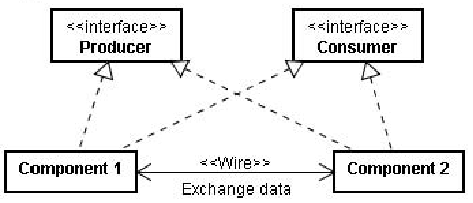
\includegraphics{Bilder/component_wire_admin.pdf}}
	\caption{Producer-Consumer Connection}
	\label{fig:component_wire_admin}
\end{figure}

As the Wire Admin and the Component Wire Admin respectively do not make any constraints on the data
exchange format, an XML based solution would be applicable for the Component Framework and the Wire
Admin Service as well, but was not implemented within the context of this master thesis.

Summing up, the Wire Admin service provides methods for exchanging data and hence realizes the
data processing part of Requirement 2, but also assumes a stronger connection and dependency between
components.

\paragraph{Event Admin Service}
\label{sec:event_admin}
The Event Admin Service provides the functionality for sending and receiving events throughout the
OSGi Framework and for realizing Requirement 8 ``Event Management''. In order to use these methods,
the Equinox implementation of the Event Admin Service has to be installed and started within the
framework. After the successful launch of the bundle, the Event Admin can be requested at the
service registry and used.

If a bundle or component respectively wants to receive and handle events, the Event Handler interface
has to be implemented and the appropriate class has to be registered at the registry. In order to
filter the events that are received by the Event Handler, the registration method takes an additional
parameter, which contains a list of properties. One of these properties defines the so-called topics,
which are nothing else than unique event identifiers within the Component and OSGi Framework
respectively, and therefore allow the filtering of single events or even sets of events.

As events are most commonly used to inform interested components about every kind of ``changes'', the
amount of information or data that is transferred is rather small. That means that the Event Admin
Service is not intended for exchanging bigger amounts of data. This is the place where the Wire Admin
Service comes into play.

\subparagraph{Event Information - An Extension to the Event Admin Service}
The event management system within the OSGi Framework requires event publishers and event
consumers, so-called ``Event Handlers''. In order to receive and process events from components,
which are unknown to the event handler, the sending component has to provide information about
them. For this purpose the ``Event Information Service'' was implemented.

That means that every component within the Component Framework, which wants to send events, has to
implement an ``Event Information'' object, which exposes human readable information about the
events, and register it at the service registry. The event information specifies the previously
described event topic, which is used as event identifier and various properties, which provide
additional information or data about when the event exactly is fired and how to handle it.

Figure \ref{fig:event_information_display} displays a simple example for a calculation result
event, which contains the name, description and topic of the event as well as the ``calculation
result'' property with its description, the identifying key, the default value and the type of the
value.

\begin{figure}
	\centering
		\fbox{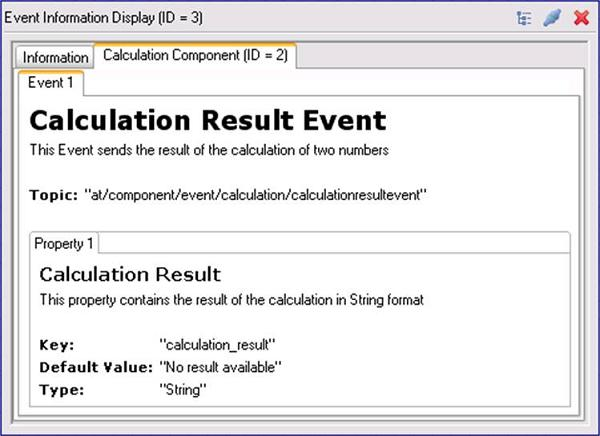
\includegraphics[width=0.6\textwidth]{Bilder/event_information_display.jpg}}
	\caption{Event Information Display}
	\label{fig:event_information_display}
\end{figure}

\subsubsection{Component Service (Requirements 4, 6 and 7)}
The ``Component Service'' finally constitutes the most powerful tool and provides a kind of management
agent (see Section \ref{label_life_cycle_layer}) for the Component Framework.

First of all this service recognizes all components and their bundles respectively which are started
with the OSGi Framework. As a second feature it provides methods for installing and uninstalling
component bundles as well as starting and stopping component instances (cf. Requirement 4 ``Running
multiple Instances of a Block''). The framework also takes care of the parent child relationship of
components and stops all child components as soon as a parent component is stopped. That means that
the component service provides a life-cycle management for components, enables the hot deployment
of new components within the Component Framework (cf. Requirement 7 ``Hot Deployment and Life-cycle
Management'').

Furthermore, the component service exposes methods for creating, saving, loading and deploying
projects. That means that the end user can reuse projects within other projects. Hence, Requirement
6 ``Reusability of Groups'' (see Section \ref{chapter:requirements}) is fulfilled and the monitor
for multiple airplanes (see Section \ref{sec:scenario}) can be implemented by first of all creating
a project for a single airplane and then integrating multiple instances of this project within a
bigger project which is adaptable to an arbitrary number of airplanes.

Another important aspect to mention about the component service and the saving
and loading of projects is, that every component can save data for reinitializing
the component during the loading process of a project. Two methods have to be
implemented to get this functionality. One for saving the data, which is called
during the saving process of the project and one for initializing the component.

As every service that is registered at the OSGi Service Registry (see Section
\ref{label_osgi_framework}) the Component Service is available throughout the entire OSGi as well as
Component Framework. Therefore, the exposed methods can be accessed by every component and enable
them to control the framework. As a second consequence the framework is absolutely independent of it's
graphical representation and the user interface. That means that the user interface which was
designed for the master thesis is just one simple example of doing it and therefore can be easily
enhanced or replaced.

\subsubsection{Component Log Service (Requirement 9)}
The ``Component Log Service'' encapsulates the log service of Eclipse Equinox and provides a simple interface for
logging all kinds of information (cf. Requirement 9 ``Logging''). It instantiates a logger which
writes the information into a log-file, which is located within the program folder. Additionally it is possible to implement
the ``IComponentLogService'' interface and add a different kind of logger, which for example prints
the information onto the console or updates the user interface of a running component.

\subsection{Extending the Component Framework (Requirement 3)}
\label{sec:extensibility}

This section deals with the development of custom components which can be managed by the Component
Framework, exchange data with other components and process events (cf. Requirement 3
``Extensibility'').

\subsubsection{Introduction}
To simplify the process of developing new components, which run within the
implemented framework, a ``New Component''-Wizard is provided as
Eclipse plug-in (see Figure \ref{fig:new_component_wizard}). This wizard only needs few inputs and
creates an Eclipse plug-in project targeted to the chosen OSGi Framework, which already
includes the basic Java classes, needed for a simple component (see Figure
\ref{fig:new_component_wizard_class_diagram}).

\begin{figure}
	\centering
		\fbox{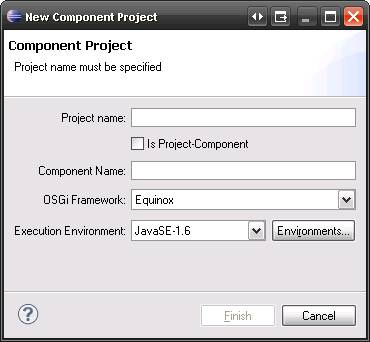
\includegraphics[width=0.6\textwidth]{Bilder/new_component_wizard.jpg}}
	\caption{New Component Wizard}
	\label{fig:new_component_wizard}
\end{figure}

\begin{figure}
	\centering
		\fbox{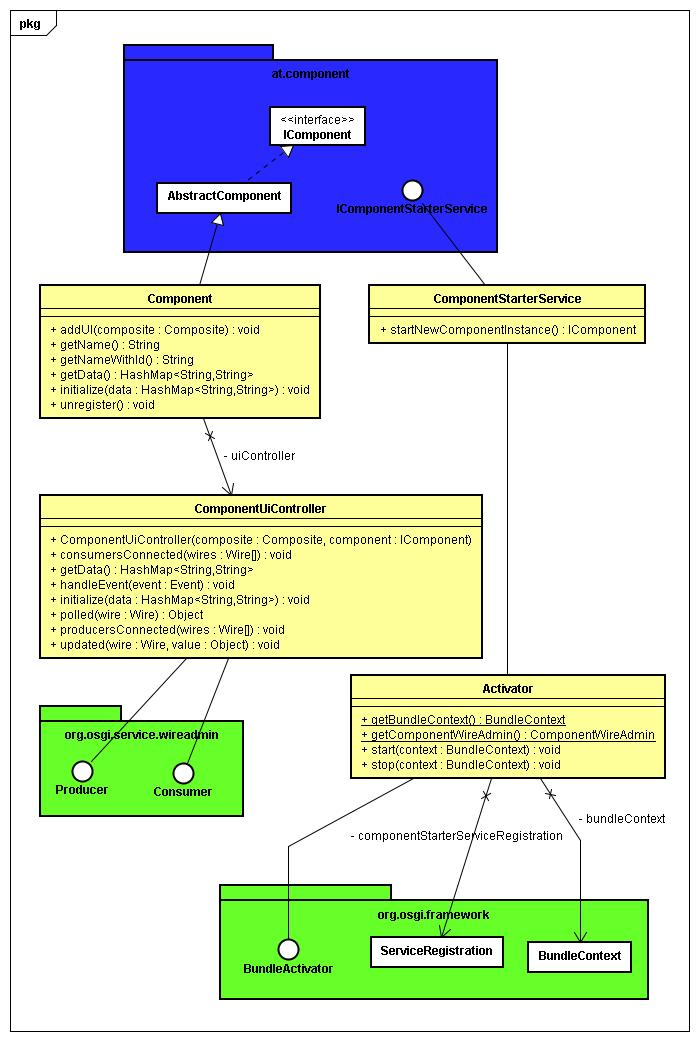
\includegraphics[width=0.8\textwidth]{Bilder/new_component_wizard_class_diagram.jpg}}
	\caption{New Component Wizard - Class Diagram}
	\label{fig:new_component_wizard_class_diagram}
\end{figure}

The Activator class implements the Bundle Activator interface of the OSGi
Framework and is the first class to be called by the framework during the
starting process of a bundle. Therefore, this class constitutes the perfect
place for registering the Component Starter Service, which is needed to start multiple instances of
a component, at the Service Registry (see Section \ref{label_osgi_framework}).

The ``Component'' class constitutes the main class of a component
implementation and provides fields for storing the name and the id of a
component, in order to identify the component instance within the running OSGi
Framework.

Furthermore, it is assumed that every component provides some
kind of user interface. Therefore, the component class provides a single
method, called ``addUI'', which provides a composite as parameter. This composite
constitutes the parent of the components user interface and hence is the place
to position buttons, input fields and all the other controls that are needed
to interact with the component. The applied mechanism can be compared with
viewparts in the RCP system of Eclipse \cite{eclipse_rcp}.

\subsubsection{Implementing the component}
\label{sec:component_implementation}
The starting point for implementing a new component is the
``ComponentUiController'' class, where the user interface class should be
instantiated (see Figure \ref{fig:new_component_wizard_class_diagram}). From that point onward
creating a component is like implementing a normal Java application according to the model-view-controller pattern.
Neither using multiple bundles for one component nor outsourcing a data model
for multiple components into a single bundle is a problem.

Therefore, simple data-display interfaces, like for example a component, which displays information
about the crew of a flight, can be done without using the Event Admin or the Component Wire Admin
(see Sections \ref{sec:event_admin} and \ref{sec:wire_admin}). As soon as a component
should react to some kind of events other components produce, or process data, which other
components are sending, these services have to be integrated and a better understanding of the OSGi
Framework is required. Nevertheless, the classes which are created by the ``New Component''-Wizard
and the services which are provided by the Component Framework -- like the adapted and extended
Wire Admin and Event Admin services -- already implement the necessary methods and just have to be
applied correctly.